%%
% This file is part of the User's Guide to RSS
% It contains the appendix for scaling tests
%%

\section{Scaling Tests}
\subsection{Internal Comparison}

We present early performance results of \RSS. The goal of the performance tests was to find out how the software scales with the number of simulated robots and specifically, which parts of the simulation take the most time to compute. All measurements have been taken on a Windows Vista PC with the following hardware: Intel Core 2 Duo at 2,53\,Ghz and 4\,GB DDR3 Ram at 1066\,Mhz. The code has been compiled using {\sffamily MinGW GCC 3.4.5}.

At all times, the visualization component of \RSS has been switched on. It runs in its own thread and consumes world information objects generated by the actual simulation kernel. To get an idea of the impact of visualization on the performance as a whole, we independently measured how long setting up each rendering frame takes. In between each frame, a variable amount of simulation time passes by, this amount is referred to as processing time. Figure~\ref{pic:scaling:render} shows that rendering one frame increases linearly with the amount of robots. At the target of 1000 robots it takes about 0.01 seconds. 

\begin{figure}[p]
	\begin{center}
	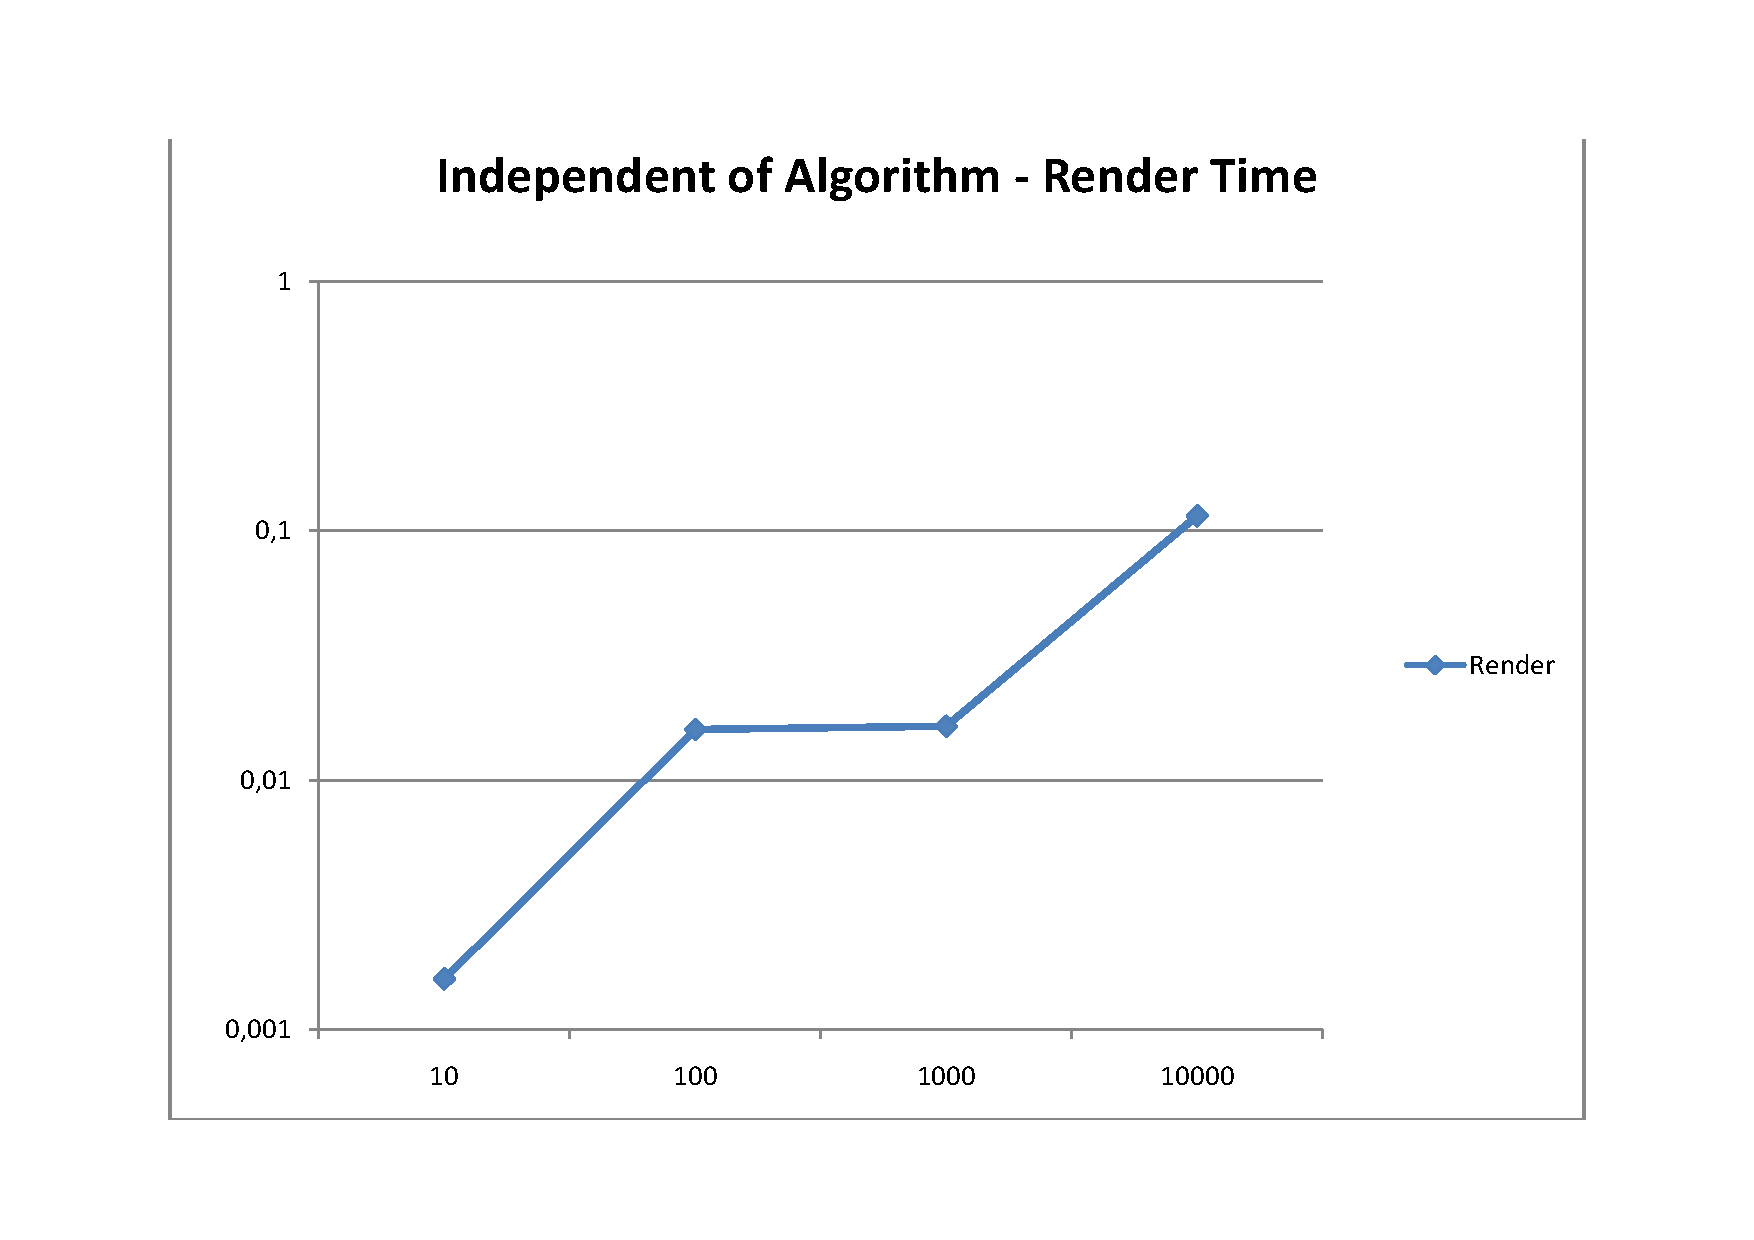
\includegraphics[width=0.8\textwidth]{scaling-render}
	\caption{Scaling test of rendering}
	\label{pic:scaling:render}
	\end{center}
\end{figure}

In the synchronous time model, each simulation step consists of updating all robots views (look event), executing each robots algorithm on that view (compute event) and then handling each robot's request to the world state (handle request event). We measured the computation time for each of these three events. The figures given represent the average time for one event after 33 steps have been simulated.

We first look at the simplest case when no algorithm at all is loaded onto the robots and they receive the global view. All robots are distributed randomly in space and receive random velocity and acceleration. Figure~\ref{pic:scaling:noglobal} tells us that Look and Request events have similar computation times and stay constant regarding the total number of robots. The compute events take almost no time and can be disregarded here. Specifically, Look and Request executed in respectively 0.15 and 0.34 seconds which results in around 0.5 seconds for a simulation step. Note that the robots actually do not return any requests so that this time can probably be regarded as overhead for copying data around.

\begin{figure}[p]
	\begin{center}
	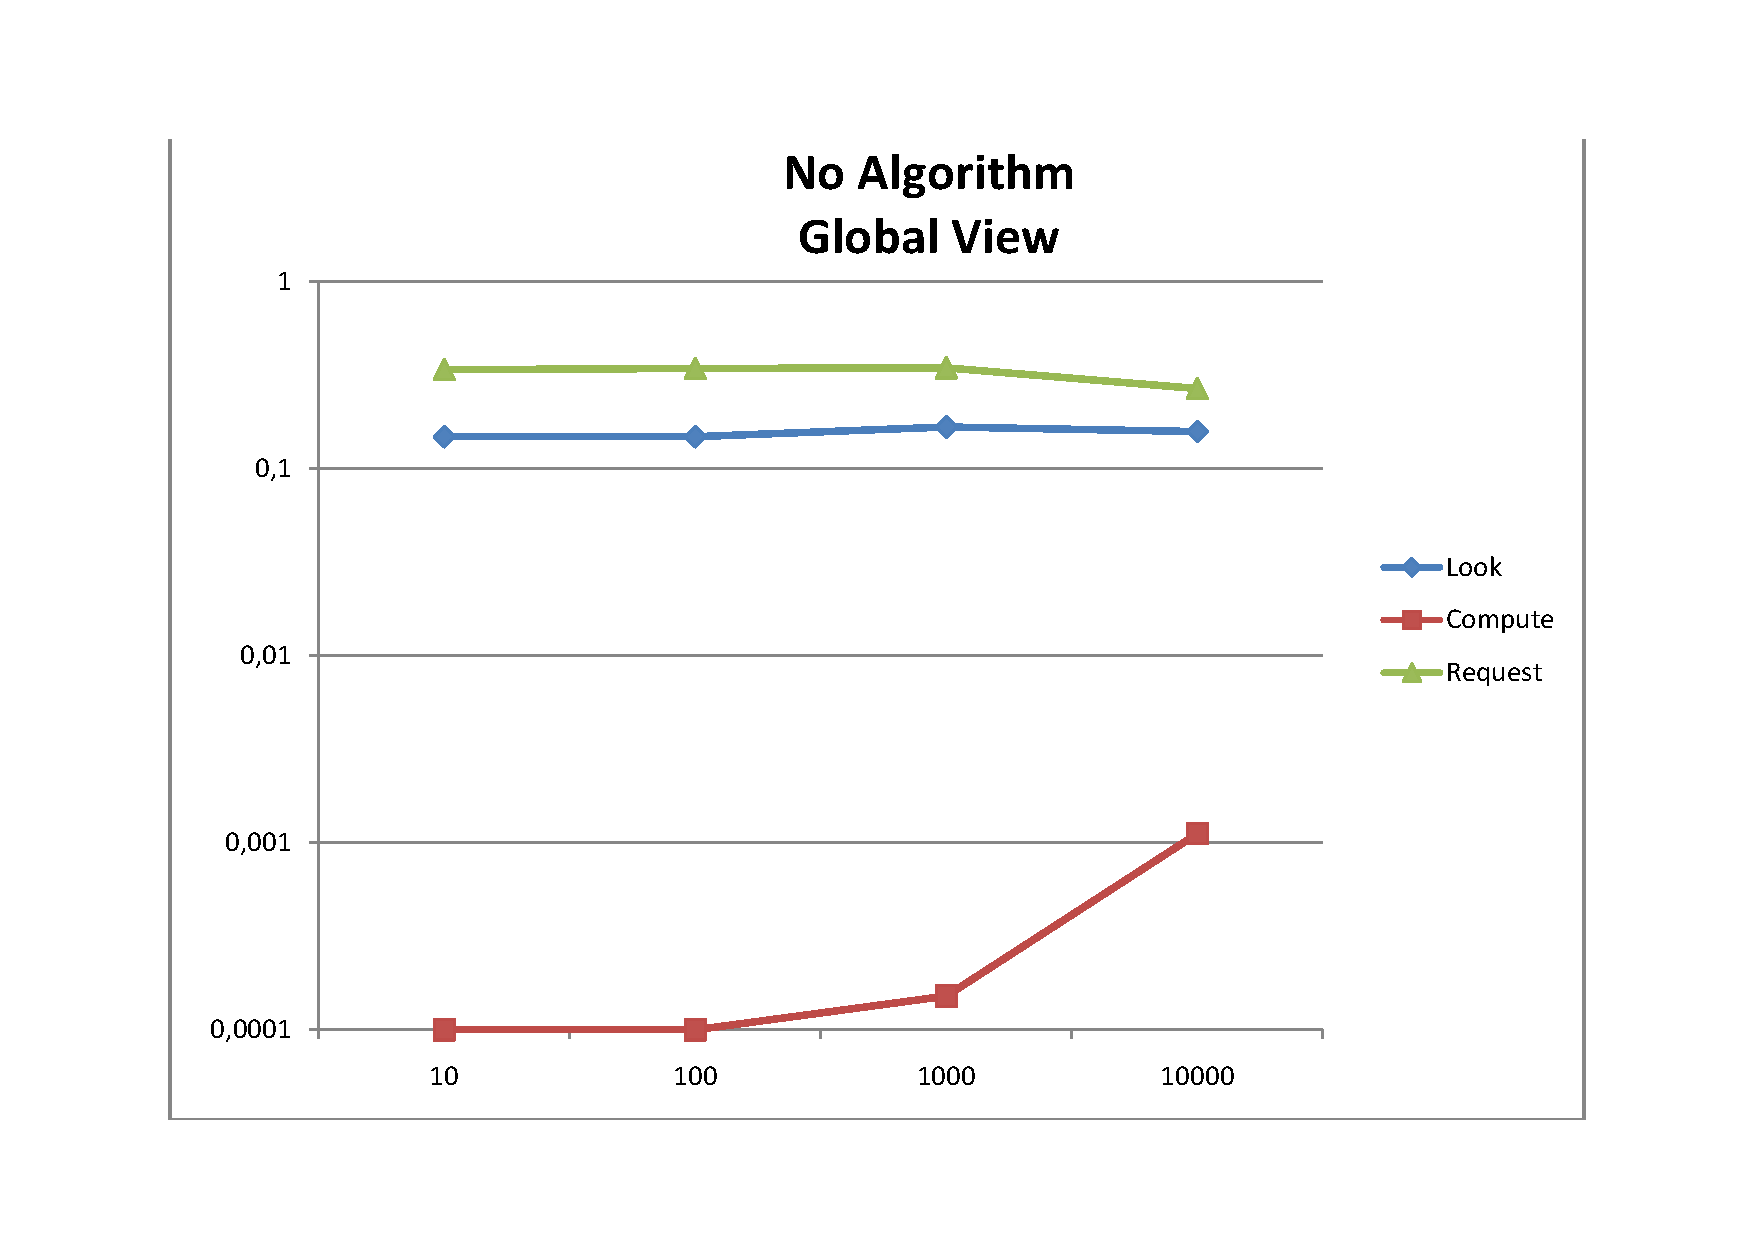
\includegraphics[width=0.8\textwidth]{scaling-no-global}
	\caption{Scaling test -- no algorithm and global view}
	\label{pic:scaling:noglobal}
	\end{center}
\end{figure}

Now we consider the Circle algorithm, specified in \texttt{circle.lua}. Here, every robot calculates the center point of all visible robots and generates a velocity request so that it rotates around the center. The robots form a rotating ring. It has been tested with global (one huge ring) and local view (several smaller rings).

Figure~\ref{pic:scaling:circleglobal} shows how performance scales in this scenario. The three different event types behave very differently. The compute event has a computation time $\mathbb{O}(n^2)$ where $n$ is the number of robots. This should be expected, as each robot regards each other in the computation of the center point. Surprisingly, the times for look and request actually decrease. When simulating 1000 robots, compute is the dominant term as each event takes 13 seconds to execute, compared to 0.010 and 0.014 for look and request respectively.

Consider the same algorithm with only a local view. We use the spheric view with a radius of 3. As it can be seen in Figure~\ref{pic:scaling:circlelocal}, the different types of events scale similarly, however in a different relation to each other. Look and request events take the same time as when using global view, which means that the octree implementation is so efficient that it is not slower than simply copying all the robots. Compute events however only take 0.94 seconds. This is due to the fact that now every robots consider only neighboring robots for calculating the center point.

\begin{figure}[p]
	\begin{center}
	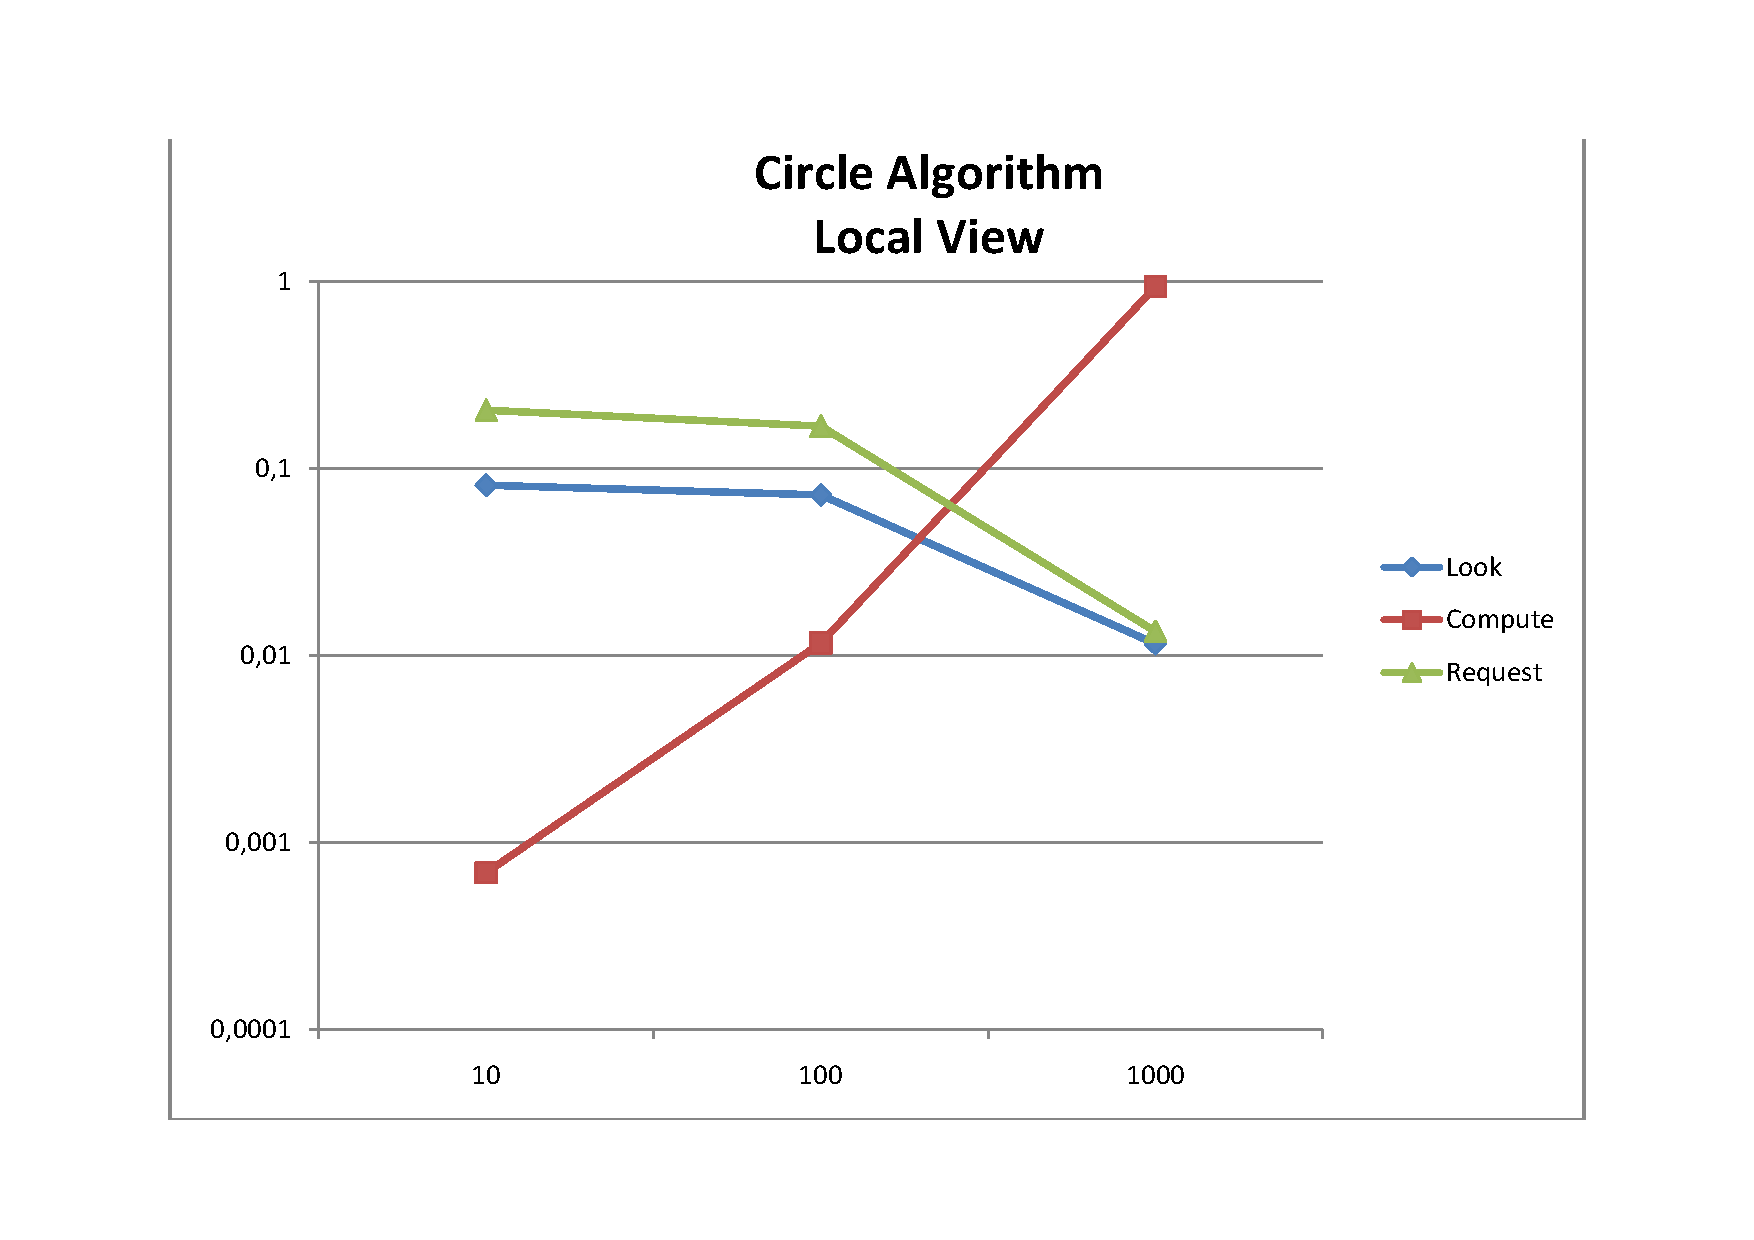
\includegraphics[width=0.8\textwidth]{scaling-circle-local}
	\caption{Scaling test -- circle local}
	\label{pic:scaling:circlelocal}
	\end{center}
\end{figure}

\begin{figure}[p]
	\begin{center}
	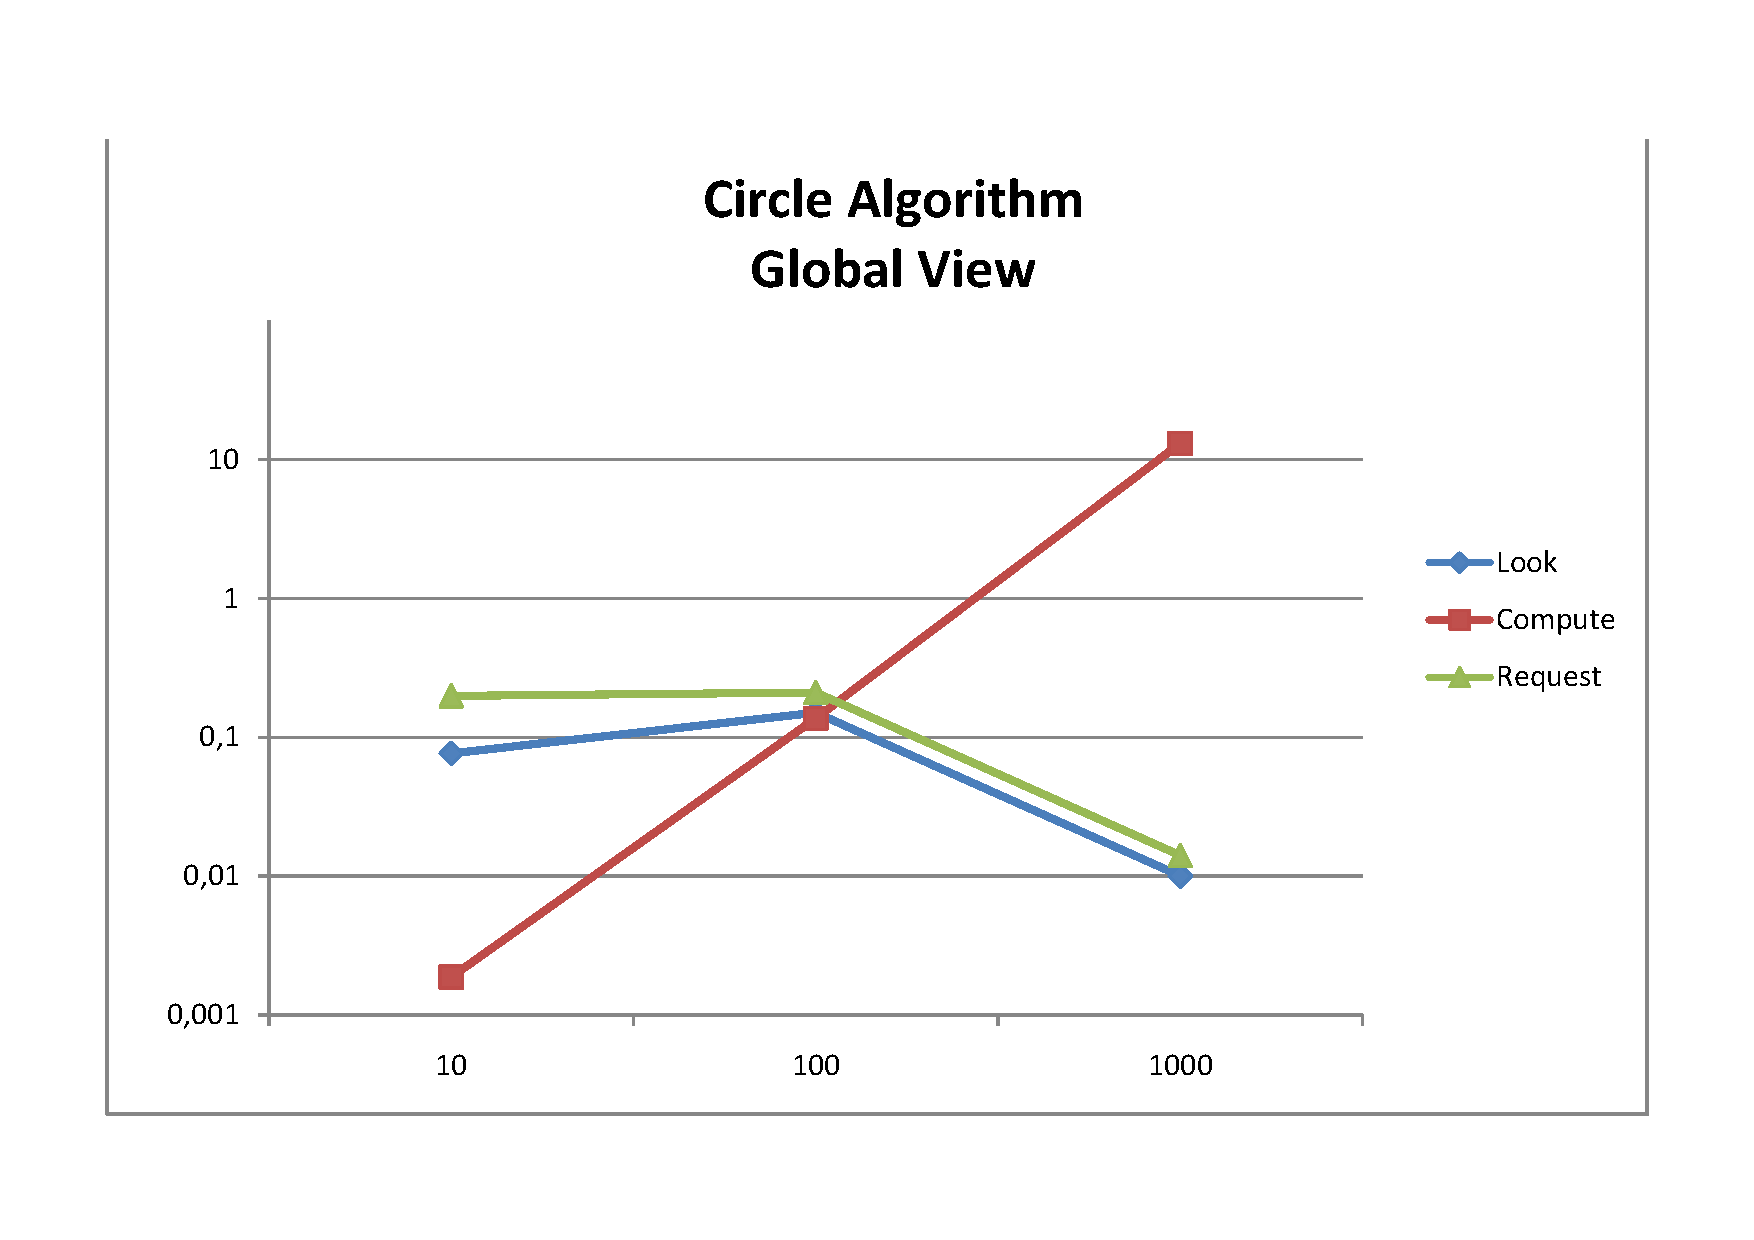
\includegraphics[width=0.8\textwidth]{scaling-circle-global}
	\caption{Scaling test -- circle global}
	\label{pic:scaling:circleglobal}
	\end{center}
\end{figure}

\subsection{Further Results}
In this section, we present results based on a late version of \RSS, specifically SVN Version 1133. We focus on verifying the earlier results and give stronger evidence, while only regarding the overall performance rather than individual parts of the software.

We have varied the amount of robots in the simulation and ran the target position algorithm. That is, each robot computes a target position (specifically, \textsc{RMinRect}) and attempts to jump to it. We iterate this \LCM cycle 500 times and take the average. Initially, the robots have been positioned uniformly within a cube with edge length $n$, where $n$ is the number of robots. The robots operate with global view and the synchronous time model. For details, refer to the theory documents. Each simulation run has been repeated 5 times.

\begin{figure}[p]
	\begin{center}
	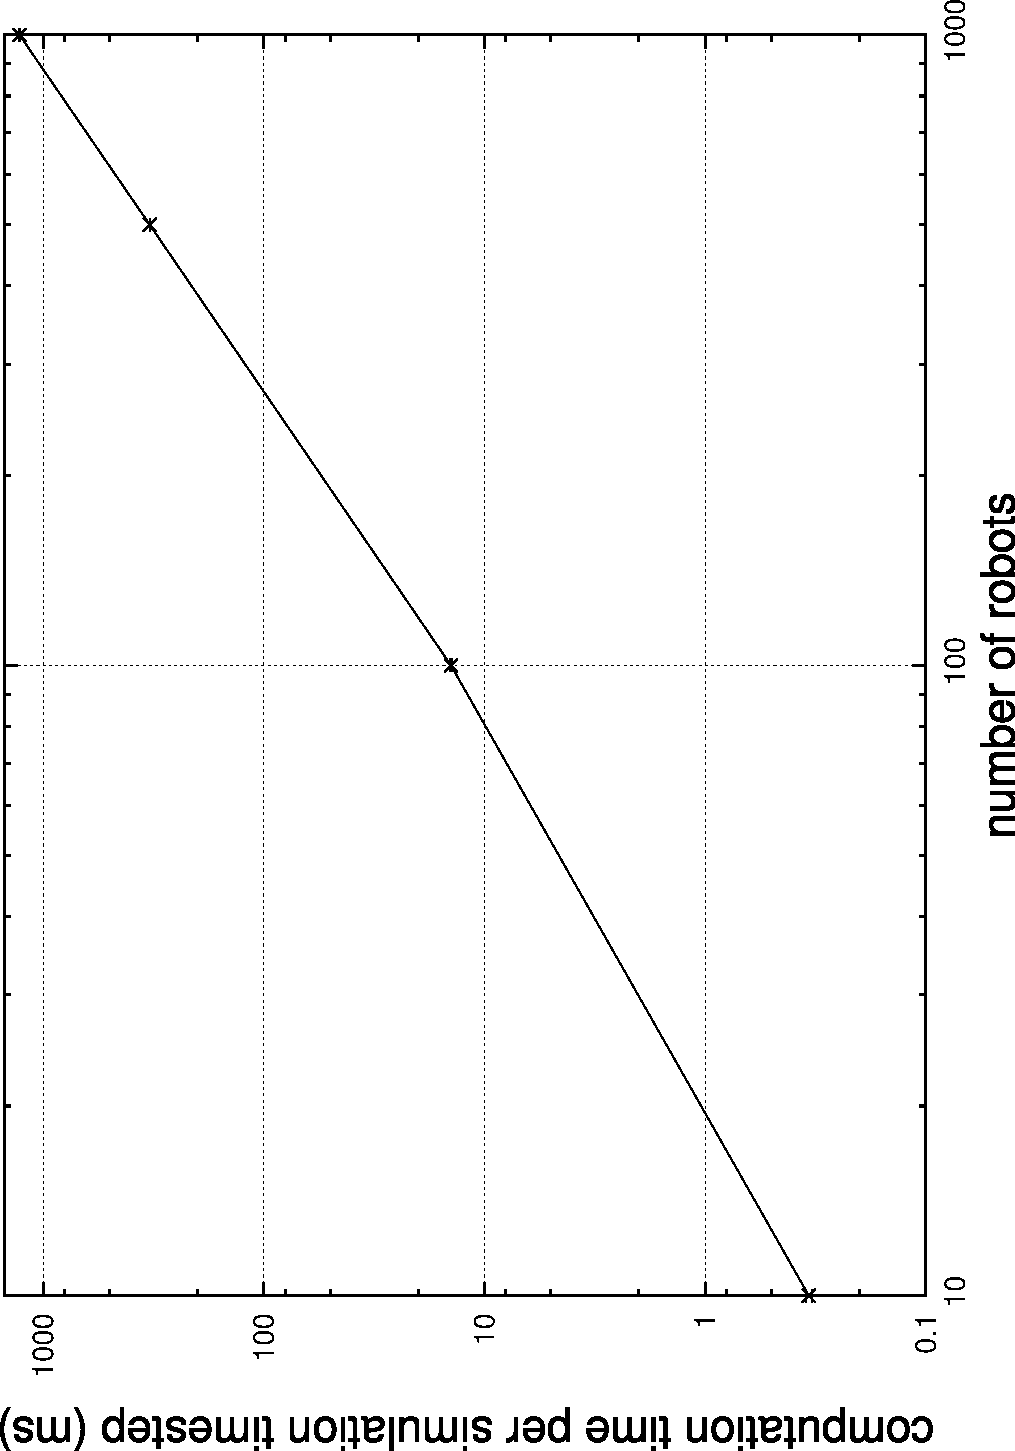
\includegraphics[width=0.8\textwidth]{scaling-rminrect}
	\caption{Scaling test -- performance depending on number of robots. The error bars illustrate the 0.9 confidence interval. Note the logarithmic axis scales.}
	\label{pic:scaling:rminrect}
	\end{center}
\end{figure}

As figure \ref{pic:scaling:rminrect} illustrates, we confirm that the computation time is $\mathbb{O}(n^2)$. Furthermore, the confidence intervals are very small, indicating that our results are dependable.